\documentclass[a4paper,14pt]{extarticle}

\usepackage[utf8x]{inputenc}
\usepackage[T1]{fontenc}
\usepackage[russian]{babel}
\usepackage{hyperref}
\usepackage{indentfirst}
\usepackage{here}
\usepackage{array}
\usepackage{graphicx}
\usepackage{grffile}
\usepackage{caption}
\usepackage{subcaption}
\usepackage{chngcntr}
\usepackage{amsmath}
\usepackage{amssymb}
\usepackage{pgfplots}
\usepackage{pgfplotstable}
\usepackage[left=2cm,right=2cm,top=2cm,bottom=2cm,bindingoffset=0cm]{geometry}
\usepackage{multicol}
\usepackage{multirow}
\usepackage{titlesec}
\usepackage{listings}
\usepackage{color}
\usepackage{longtable}
\usepackage{enumitem}
\usepackage{cmap}
\usepackage{tikz}

\usetikzlibrary{shapes,arrows}

\definecolor{green}{rgb}{0,0.6,0}
\definecolor{gray}{rgb}{0.5,0.5,0.5}
\definecolor{purple}{rgb}{0.58,0,0.82}

\lstset{
	extendedchars=\true,
	keepspaces=true,
	language={bash},
	inputpath={logs},
	backgroundcolor=\color{white},
	commentstyle=\color{green},
	keywordstyle=\color{blue},
	numberstyle=\scriptsize\color{gray},
	stringstyle=\color{purple},
	basicstyle=\small,
	breakatwhitespace=false,
	breaklines=true,
	captionpos=b,
	keepspaces=true,
	numbers=left,
	numbersep=5pt,
	showspaces=false,
	showstringspaces=false,
	showtabs=false,
	tabsize=8,
	frame=single,
}

\renewcommand{\le}{\ensuremath{\leqslant}}
\renewcommand{\leq}{\ensuremath{\leqslant}}
\renewcommand{\ge}{\ensuremath{\geqslant}}
\renewcommand{\geq}{\ensuremath{\geqslant}}
\renewcommand{\epsilon}{\ensuremath{\varepsilon}}
\renewcommand{\phi}{\ensuremath{\varphi}}
\renewcommand{\thefigure}{\arabic{figure}}
\def\code#1{\texttt{#1}}

\titleformat*{\section}{\large\bfseries} 
\titleformat*{\subsection}{\normalsize\bfseries} 
\titleformat*{\subsubsection}{\normalsize\bfseries} 
\titleformat*{\paragraph}{\normalsize\bfseries} 
\titleformat*{\subparagraph}{\normalsize\bfseries} 

\counterwithin{figure}{section}
\counterwithin{equation}{section}
\counterwithin{table}{section}
\newcommand{\sign}[1][5cm]{\makebox[#1]{\hrulefill}}
\newcommand{\equipollence}{\quad\Leftrightarrow\quad}
\newcommand{\no}[1]{\overline{#1}}
\graphicspath{{figs/}}
\captionsetup{justification=centering,margin=1cm}
\def\arraystretch{1.3}
\setlength\parindent{5ex}
\titlelabel{\thetitle.\quad}

\setitemize{itemsep=0em}
\setenumerate{itemsep=0em}

\tikzstyle{startstop} = [
	rectangle,
	align=center,
	rounded corners,
	text width=10em,
	text centered,
	draw=black
]
\tikzstyle{process} = [
	rectangle,
	align=center,
	text width=20em,
	text centered,
	draw=black
]
\tikzstyle{decision} = [
	diamond,
	aspect=4,
	align=center,
	inner sep=0pt,
	text width=10em,
	text centered,
	node distance=5em,
	draw=black
]
\tikzstyle{line} = [
	draw=black,
	thick,
	->,
	>=stealth,
	-latex'
]

\begin{document}

\begin{titlepage}
\begin{center}
	САНКТ-ПЕТЕРБУРГСКИЙ ПОЛИТЕХНИЧЕСКИЙ УНИВЕРСИТЕТ\\ ПЕТРА ВЕЛИКОГО\\[0.3cm]
	\par\noindent\rule{10cm}{0.4pt}\\[0.3cm]
	Институт компьютерных наук и технологий \\[0.3cm]
	Кафедра компьютерных систем и программных технологий\\[4cm]
	
	Отчет по лабораторной работе\\[3mm]
	Дисциплина: <<Защита информации>>\\[3mm]
	Тема: <<Рассмотрение PGP системы GnuPG>>\\[7cm]
\end{center}

\begin{flushleft}
	\hspace*{5mm} Выполнил студент гр. 43501/3  \hspace*{1.5cm}\sign[3cm]\hfill А.В. Кнорре\\
	\hspace*{9.4cm} (подпись)\\[3mm]
	\hspace*{5mm} Преподаватель \hspace*{5.0cm}\sign[3cm]\hfill А.Г. Новопашенный\\
	\hspace*{9.4cm} (подпись)\\[5mm]
	\hspace*{11.1cm} <<\sign[7mm]>> \sign[27mm] \the\year\hspace{1mm} г.
\end{flushleft}

\vfill

\begin{center}
	Санкт-Петербург\\
	\the\year
\end{center}
\end{titlepage}
\addtocounter{page}{1}

\tableofcontents
\listoffigures
\lstlistoflistings
\newpage

\section{Цель работы}

Научиться анализировать сетевой трафик при помощи программы \code{WireShark}.

\section{Программа работы}

Проанализировать сетевой трафик:

\begin{enumerate}
	\item Протокола ARP
	\item Протокола ICMP
	\begin{itemize}
		\item \code{ping} без фрагментации
		\item \code{ping} с фрагментацией
		\item \code{traceroute}
		\item ошибка 3/1
	\end{itemize}
	\item Протокола UDP
	\item Протокола TCP
	\begin{itemize}
		\item установление соединения
		\item закрытие соединения
		\item флаг \code{RST}
	\end{itemize}
\end{enumerate}

\section{Условия сети}

Часть работы была выполнена в сети кафедры. Её конфигурация представлена в листинге \ref{lst:net-kspt}.

\lstinputlisting[caption={Конфигурация сети кафедры},label={lst:net-kspt},keywords={config},basicstyle=\scriptsize]{config_kspt.txt}


Другая часть работы была выполнена в домашней сети, конфигурация которой представлена в листинге \ref{lst:net-home}.

\lstinputlisting[caption={Конфигурация домашней сети},label={lst:net-home},keywords={config},basicstyle=\scriptsize]{config_home.txt}

\section{Протокол ARP}

Рассмотрим принцип действия протокола ARP. Выполним широковещательный ARP-запрос в домашней сети, отправив \code{ping} пакет другому узлу сети (домашняя сеть) по адресу \code{192.168.86.246}.  На рис. \ref{fig:arp-req} представлен ARP-запрос.

\begin{figure}[H]
	\centering
	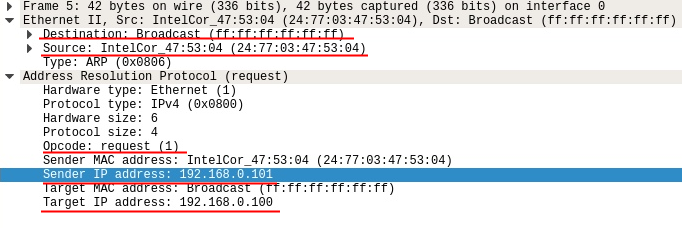
\includegraphics[width=1\textwidth]{arp-req}
	\caption{ARP-запрос}
	\label{fig:arp-req}
\end{figure}

Затем, узел сети по адресу \code{192.168.86.246} отправляет нам ARP-ответ, который представлен на рис. \ref{fig:arp-resp}

\begin{figure}[H]
	\centering
	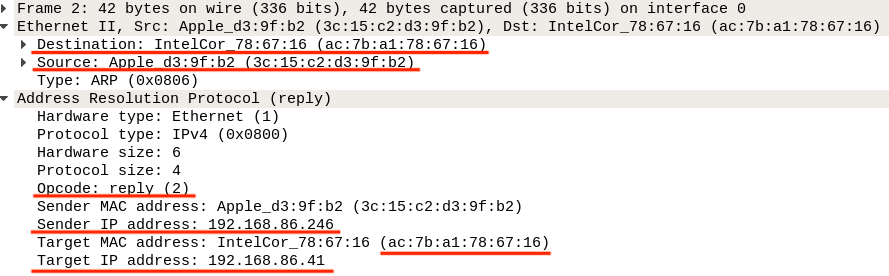
\includegraphics[width=1\textwidth]{arp-resp}
	\caption{ARP-ответ}
	\label{fig:arp-resp}
\end{figure}

\section{Протокол ICMP}

\subsection{Утилита \code{ping}}

Утилита \code{ping} отправляет ICMP эхо-запрос, на который, в случае успеха приходит ICMP эхо-ответ. Если пакет не пришел за определённое время, то удалённый хост считается недостижимым.

\paragraph{Ping без фрагментации}

Т.к. для Ethernet 2 размер MTU равен 1500 байтов (без заголовка -- 1480), то для отправки пакетов утилитой \code{ping} без фрагментации ничего не нужно делать, т.к. размер пакета по умолчанию не превышает MTU.

Отправим с помощью утилиты \code{ping} ICMP эхо-запрос сайту ok.ru (листинг \ref{lst:ping}). Он представлен на рис. \ref{fig:ping-req}.

\lstinputlisting[caption={Ping без фрагментации},label={lst:ping},keywords={ping}]{ping.txt}

\begin{figure}[H]
	\centering
	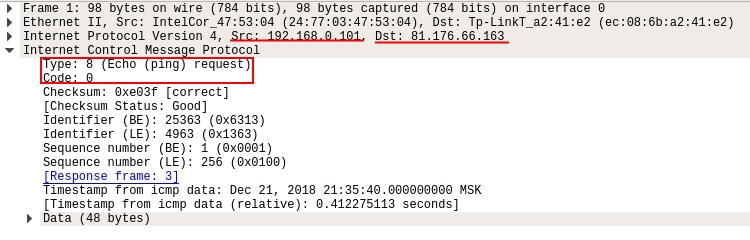
\includegraphics[width=1\textwidth]{ping-req}
	\caption{Ping ICMP эхо-запрос (без фрагментации)}
	\label{fig:ping-req}
\end{figure}

Затем нам приходит от сайта ok.ru ICMP эхо-ответ (рис. \ref{fig:ping-resp}).

\begin{figure}[H]
	\centering
	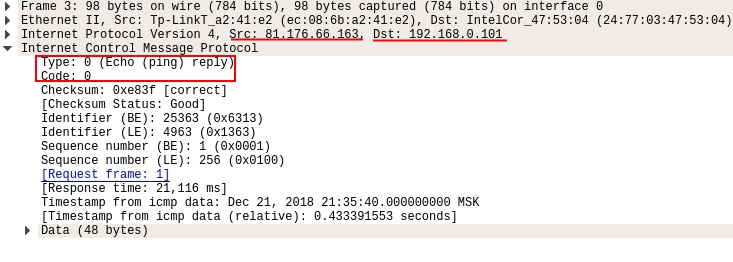
\includegraphics[width=1\textwidth]{ping-resp}
	\caption{Ping ICMP эхо-ответ (без фрагментации)}
	\label{fig:ping-resp}
\end{figure}

\newpage

\paragraph{Ping с фрагментацией}

Для достижения фрагментации пакета, зададим его размер равным 4000 байтов (листинг \ref{lst:ping-frag}).

\lstinputlisting[caption={Ping с фрагментацией},label={lst:ping-frag},keywords={ping}]{ping-frag.txt}

Отправленный пакет представлен на рис. \ref{fig:ping-req-frag}.

\begin{figure}[H]
	\centering
	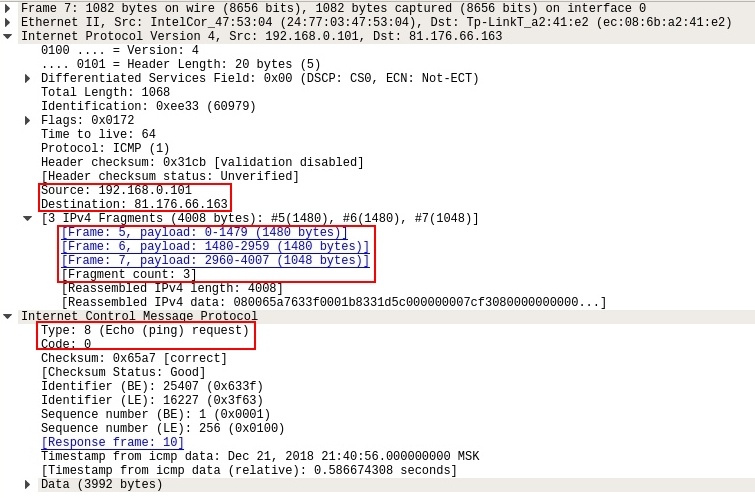
\includegraphics[width=1\textwidth]{ping-req-frag}
	\caption{Ping ICMP эхо-запрос (с фрагментацией)}
	\label{fig:ping-req-frag}
\end{figure}

Затем нам приходит от сайта ok.ru ICMP эхо-ответ (рис. \ref{fig:ping-resp-frag}).

\begin{figure}[H]
	\centering
	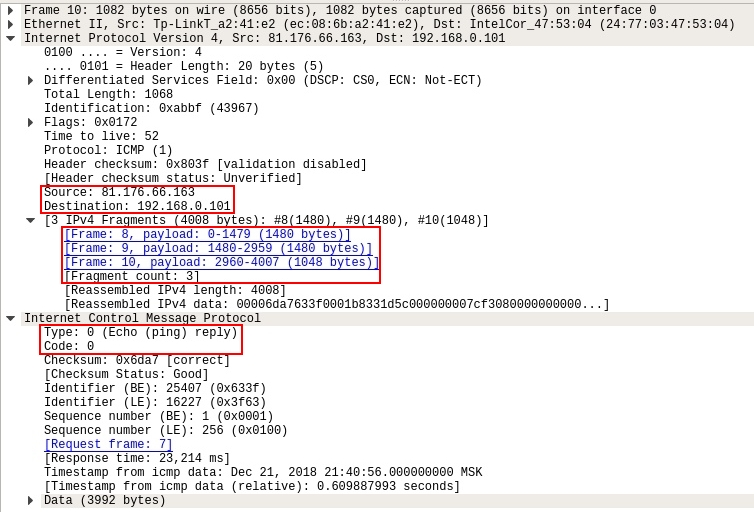
\includegraphics[width=1\textwidth]{ping-resp-frag}
	\caption{Ping ICMP эхо-ответ (с фрагментацией)}
	\label{fig:ping-resp-frag}
\end{figure}

\subsection{Утилита \code{traceroute}}\label{sec:traceroute}

Утилита \code{traceroute} отправляет ICMP эхо-запросы, инкрементируя поле TTL, пока приходят ошибки истечения TTL вместо эхо-ответа. Изначальное значение поля TTL = 1.

Выполним трассировку маршрута до сайта ok.ru (листинг \ref{lst:trace}).

\lstinputlisting[caption={Трассировка маршрута до ok.ru},label={lst:trace},keywords={traceroute}]{traceroute.txt}

В листинге видно, что удалось отследить маршрут только до маршрутизатора \code{dp-1.spbix.m100.ru}.

На рис. \ref{fig:trace1} --- \ref{fig:trace4} изображены ICMP ответы четырёх промежуточных маршрутизаторов, до которых удалось дойти.

\begin{figure}[H]
	\centering
	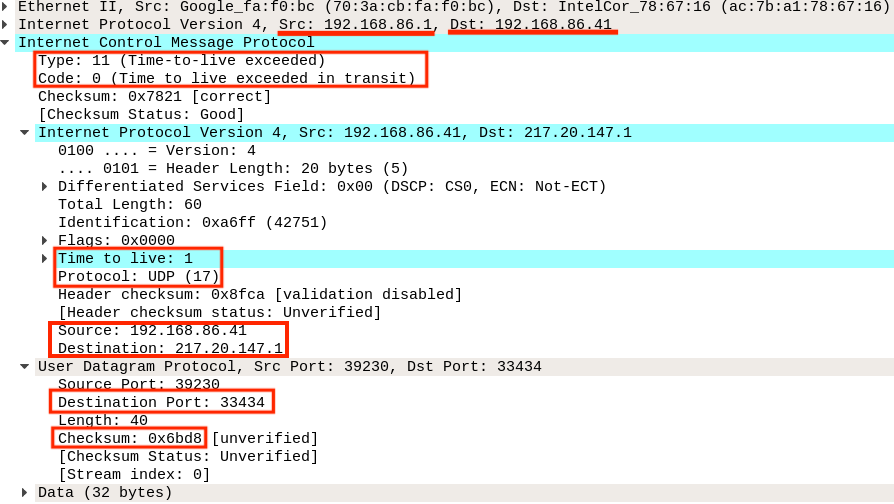
\includegraphics[width=1\textwidth]{trace1}
	\caption{ICMP ответ маршрутизатора домашней сети}
	\label{fig:trace1}
\end{figure}

\begin{figure}[H]
	\centering
	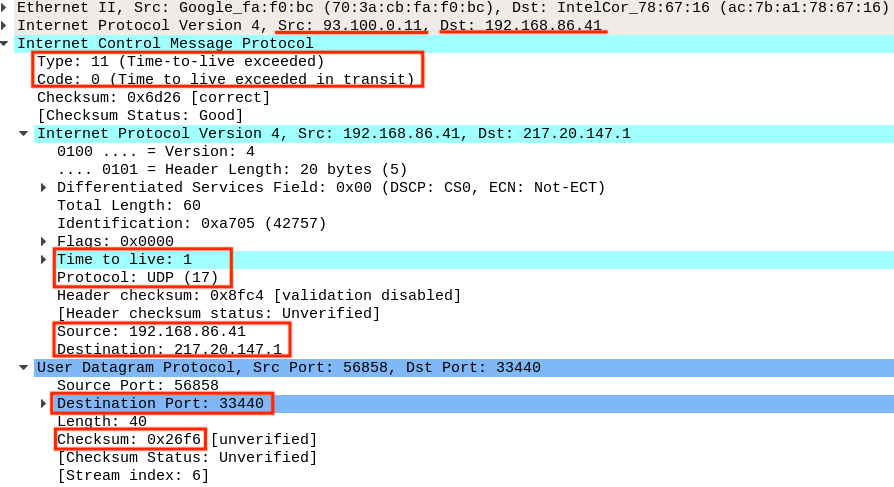
\includegraphics[width=1\textwidth]{trace2}
	\caption{ICMP ответ маршрутизатора провайдера \code{sknt.ru}}
	\label{fig:trace2}
\end{figure}

\begin{figure}[H]
	\centering
	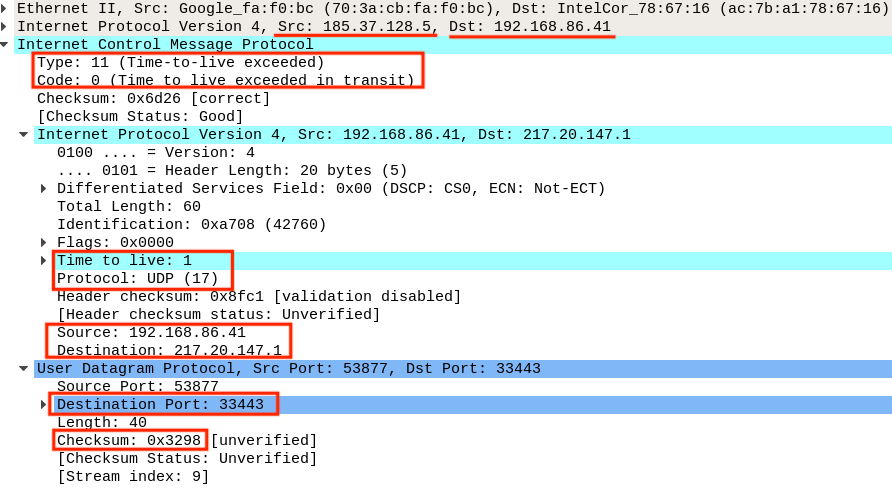
\includegraphics[width=1\textwidth]{trace3}
	\caption{ICMP ответ маршрутизатора \code{185.37.128.85}}
	\label{fig:trace3}
\end{figure}

\begin{figure}[H]
	\centering
	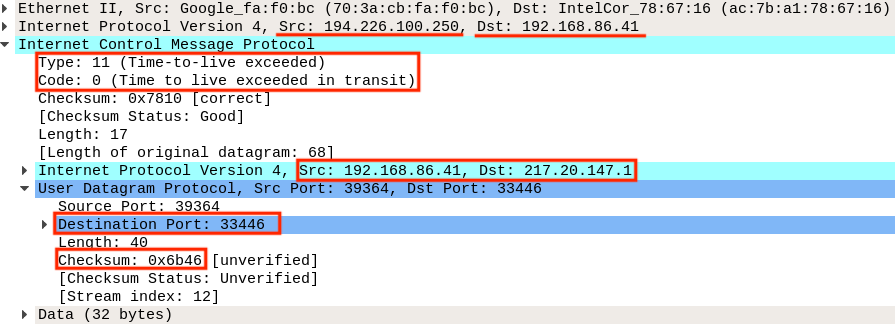
\includegraphics[width=1\textwidth]{trace4}
	\caption{ICMP ответ маршрутизатора \code{dp-1.spbix.m100.ru}}
	\label{fig:trace4}
\end{figure}

\subsection{Ошибка 3/1}

Для получения ICMP ошибки 3/1 (Хост недостижим), выполним \code{ping} хоста \code{10.1.17.3} сети кафедры. ICMP-ответ с ошибкой предствален на рис. \ref{fig:icmp31}.

\begin{figure}[H]
	\centering
	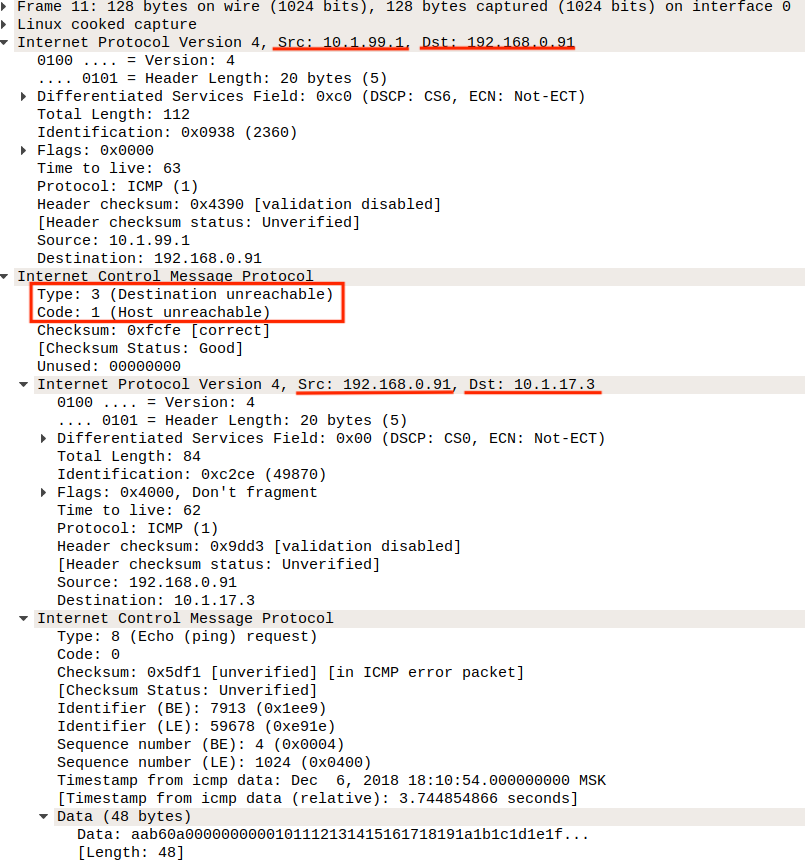
\includegraphics[width=1\textwidth]{icmp31}
	\caption{ICMP ответ 3/1}
	\label{fig:icmp31}
\end{figure}

\newpage

\section{Протокол UDP}

Развернём на хосте \code{192.168.86.246} UDP сервер на порту 1234. Затем на нашем хосте \code{192.168.86.41} запустим клиентское приложение и выполним сервер запрос. Он изображён на рис. \ref{fig:udp-req}.

\begin{figure}[H]
	\centering
	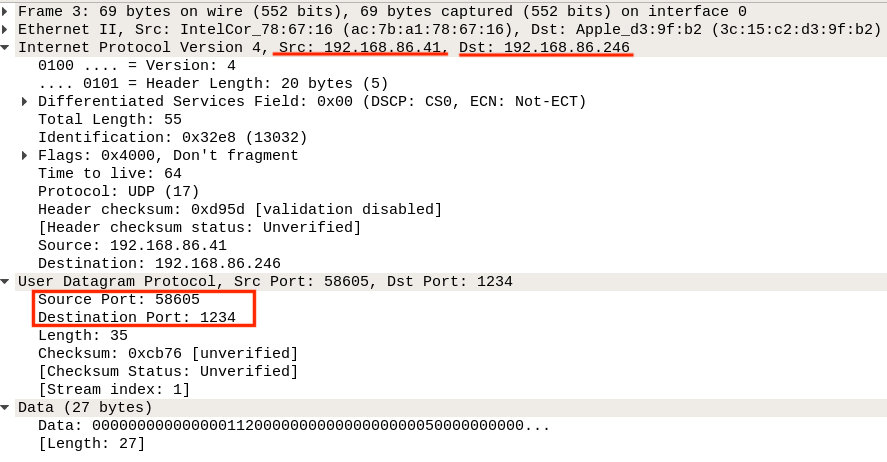
\includegraphics[width=1\textwidth]{udp-req}
	\caption{Запрос на сервер по UDP}
	\label{fig:udp-req}
\end{figure}

Сервер реализован таким образом, что на правильно сформированный запрос он отправляет ответ. Ответ представлен на рис. \ref{fig:udp-resp}.

\begin{figure}[H]
	\centering
	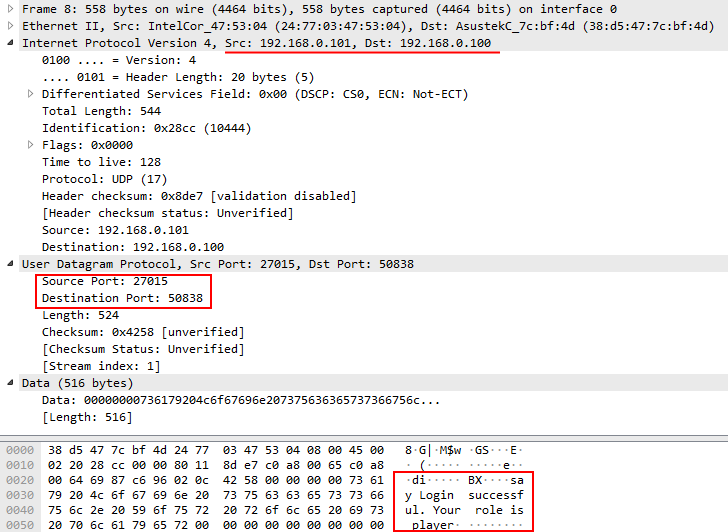
\includegraphics[width=1\textwidth]{udp-resp}
	\caption{Ответ UDP сервера}
	\label{fig:udp-resp}
\end{figure}

\section{Протокол TCP}

Развернём на хосте \code{192.168.86.246} TCP сервер на порту 1234. 

\subsection{Установление соединения}

На нашем хосте \code{192.168.86.41} запустим клиентское приложение. Оно сразу при запуске пытается установить соединение с сервером. Как видно на рис. \ref{fig:tcp-syn} -- \ref{fig:tcp-ack} соединение происходит за 3 шага:

\begin{enumerate}
	\item Клиент отправляет \code{SYN}
	\item Сервер отправляет \code{SYN} и \code{ACK}
	\item Клиент отправляет \code{ACK}
\end{enumerate}

\begin{figure}[H]
	\centering
	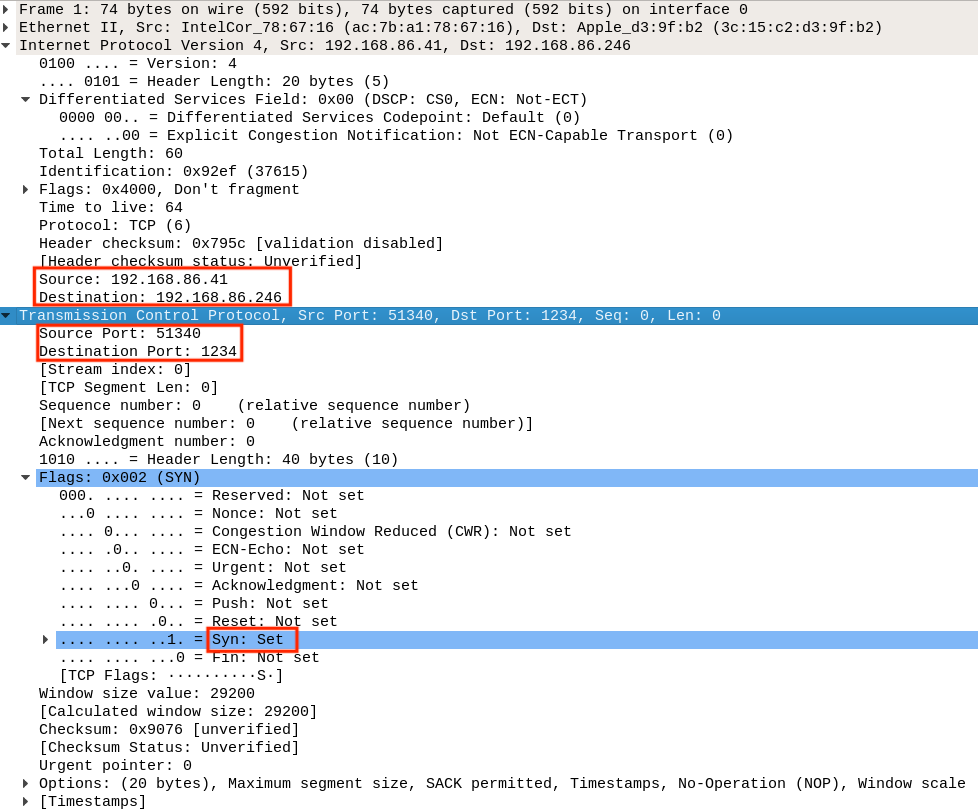
\includegraphics[width=1\textwidth]{tcp-syn}
	\caption{Отправка клиентом \code{SYN}}
	\label{fig:tcp-syn}
\end{figure}

\begin{figure}[H]
	\centering
	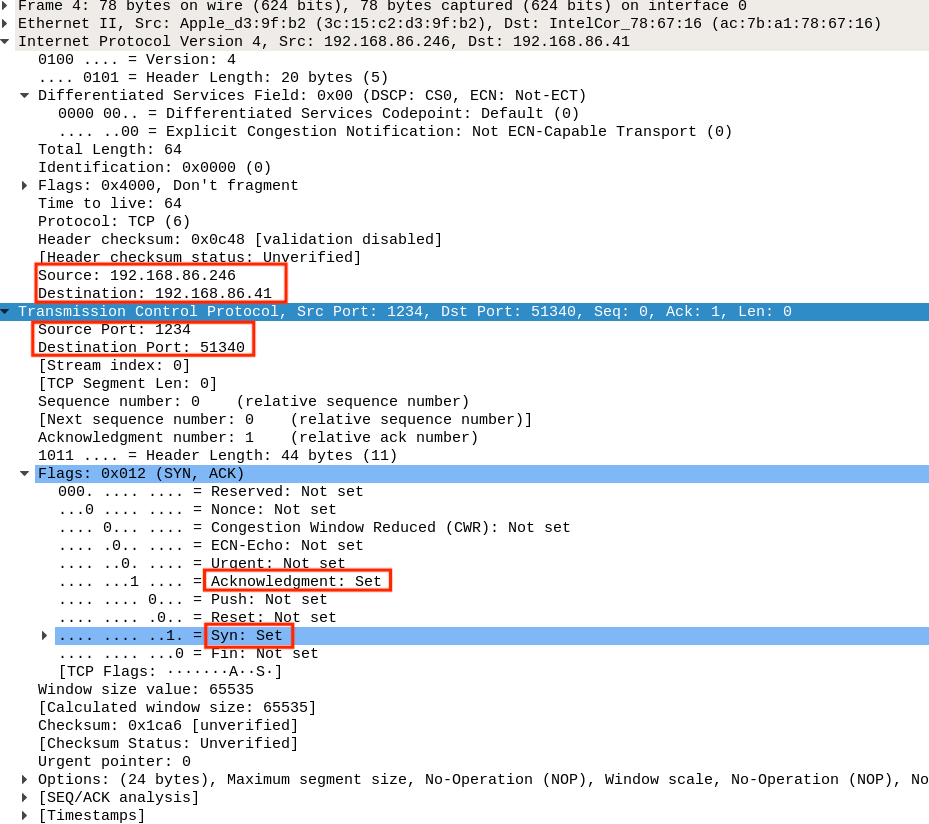
\includegraphics[width=1\textwidth]{tcp-synack}
	\caption{Отправка сервером \code{SYN} и \code{ACK}}
	\label{fig:tcp-synack}
\end{figure}

\begin{figure}[H]
	\centering
	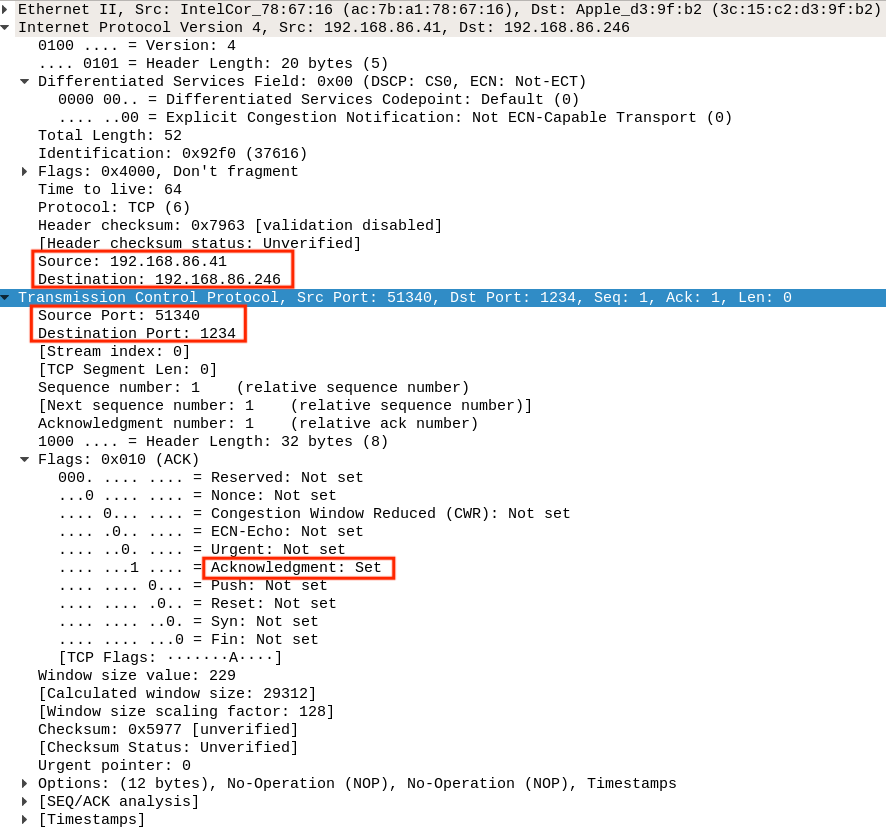
\includegraphics[width=1\textwidth]{tcp-ack}
	\caption{Отправка клиентом \code{ACK}}
	\label{fig:tcp-ack}
\end{figure}

\subsection{Закрытие соединения}

На хосте \code{192.168.86.246}, на котором развёрнут сервер инициируем разрыв соединения, отправив клиенту \code{FIN} и \code{ACK}. После этого клиент отправляет серверу \code{ACK}, и соединение считается закрытым.

На рис. \ref{fig:tcp-finack} изображён TCP-сегмент с \code{FIN} и \code{ACK}.

\begin{figure}[H]
	\centering
	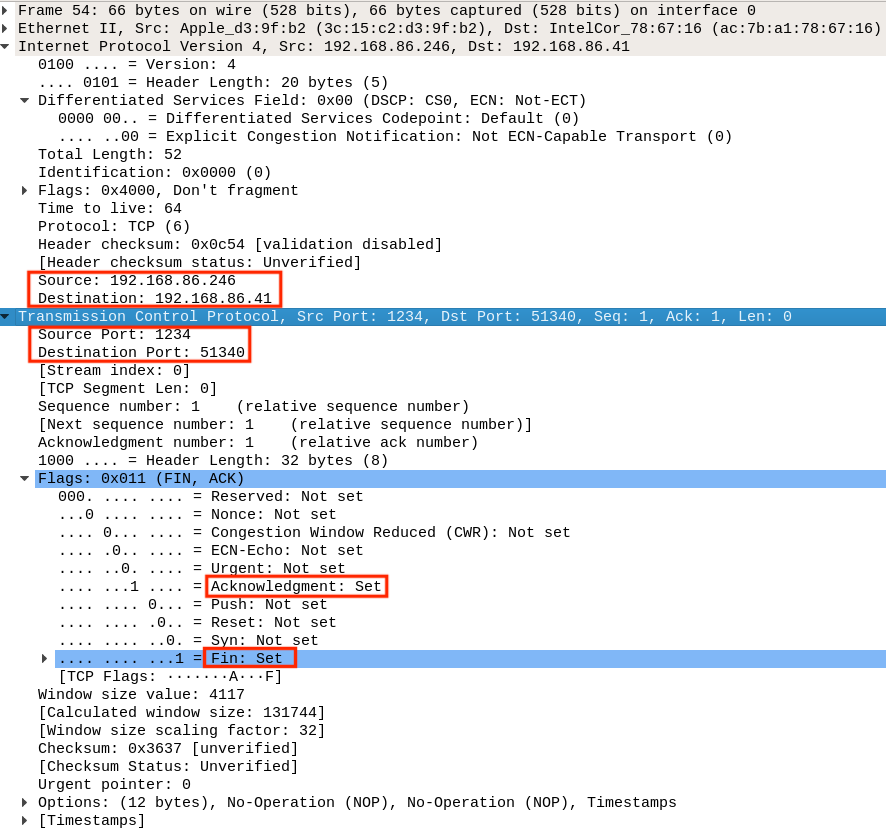
\includegraphics[width=1\textwidth]{tcp-finack}
	\caption{Отправка сервером \code{FIN} и \code{ACK}}
	\label{fig:tcp-finack}
\end{figure}

На рис. \ref{fig:tcp-finack-ack} изображён TCP-сегмент с \code{ACK}.

\begin{figure}[H]
	\centering
	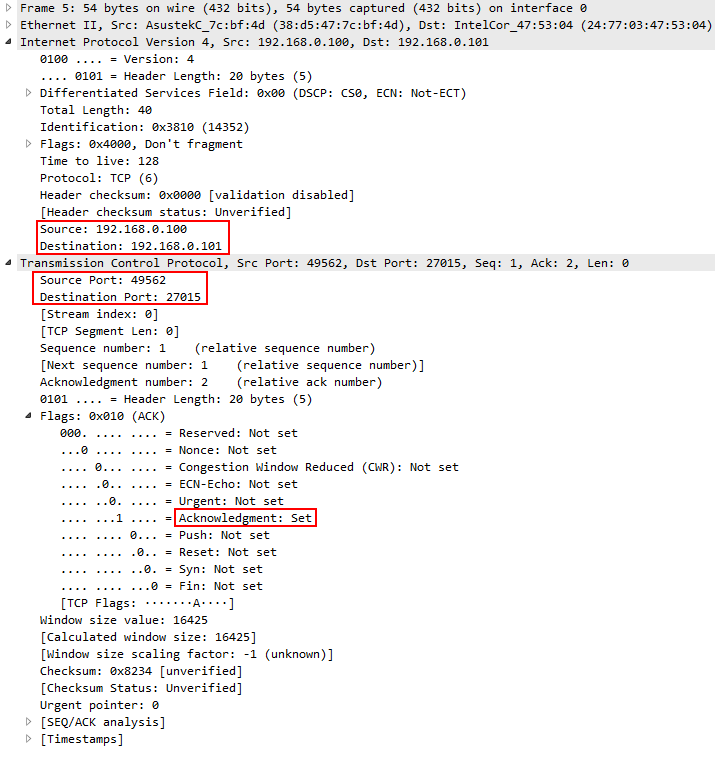
\includegraphics[width=1\textwidth]{tcp-finack-ack}
	\caption{Отправка клиентом \code{ACK}}
	\label{fig:tcp-finack-ack}
\end{figure}

\subsection{Флаг \code{RST}}

Завершим работу TCP сервера, развёрнутого на хосте \code{192.168.86.246}. После этого запустим на нашем хосте клиентское приложение, которое сразу попытается установить соединение. Но этого сделать не удаётся -- на \code{SYN} приходит \code{RST} и \code{ACK}. TCP-сегмент с \code{RST} и \code{ACK} представлен на рис. \ref{fig:tcp-rstack}.

\begin{figure}[H]
	\centering
	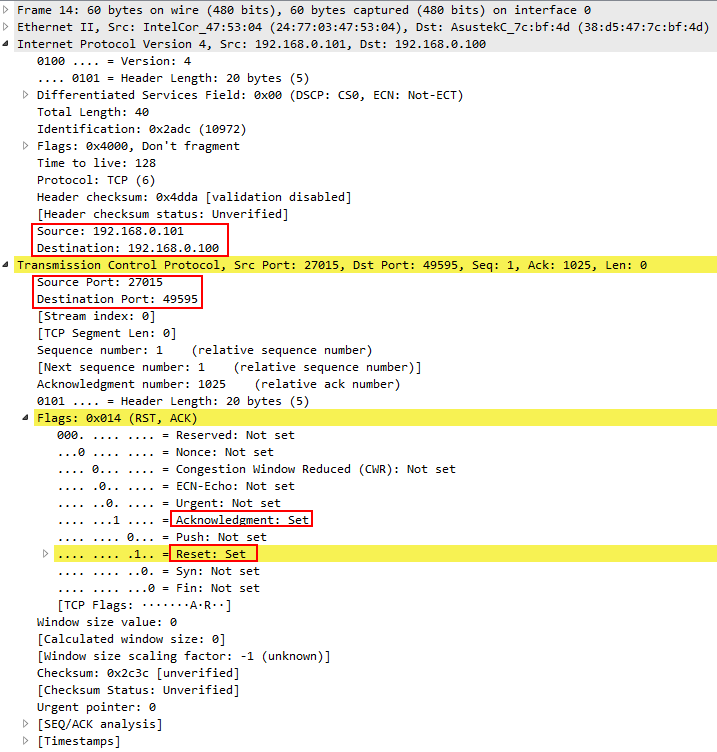
\includegraphics[width=0.9\textwidth]{tcp-rstack}
	\caption{TCP-сегмент с \code{RST} и \code{ACK}}
	\label{fig:tcp-rstack}
\end{figure}

\section{Выводы}

В ходе работы с помощью утилиты \code{WireShark} был рассмотрен трафик протоколов ARP, ICMP, UDP и TCP. Также были рассмотрены утилиты \code{ping} и \code{traceroute}, которые, используя протокол ICMP, позволяют определить достижимость удалённого хоста и трассировать маршрут до удалённого хоста соответственно.

Утилита \code{WireShark} оказалась очень удобным инструментом для анализа трафик, потому что она позволяет гибко фильтровать трафик, например, по протоколу.

Главный вывод заключается в том, что внутри одной сети можно просмотреть абсолютно весь трафик, и если протокол не использует шифрование, как, например, какой-либо строковый протокол на основе TCP, то данные пересылаемые с его помощью легко прочитать, чем могут воспользоваться злоумышленники.

\section{Приложение}

\subsection{Дополнение к опыту с утилитой \code{traceroute}}

Утилита \code{tracert} (которая установлена в ОС Windows), в действительности работает по принципу, описанному в разделе \ref{sec:traceroute}, т.е, в её основе польностью лежит \code{ICMP}. А опыт на самом деле проводился на хосте с ОС Linux c помощью похожей утилиты -- \code{traceroute}. Назначение у неё такое же как и у \code{tracert}, а реализация другая.

\code{traceroute} основана не на отправке ICMP эхо-запросов, а на отправке UDP фрагментов и получения сообщения о доступности/достижимости порта. Host генерирует UDP фрагмент, инкапсулирует его в IP пакет и выставляет TTL=1. Первый маршрутизатор на пути, являясь транзитным узлом, ответит на данный пакет ICMP сообщением об окончании времени жизни пакета. Утилита \code{traceroute}, получив данное сообщение, указывает адрес источника ICMP пакета как адрес первого хопа. Далее процесс повторяется с инкрементированием TTL пакета. Тут встаёт вопрос --- как утилите понять, что трассировка закончена? В UDP заголовке есть поля source port и destination port. Destination порт устанавливается 33434 (это число инкрементируется с каждой попыткой). Когда пакет доходит до сервера назначения, сервер его распаковывает. Понимая, что порт, указанный в заголовке как destination port, у него закрыт, он отправляет ICMP сообщение (ICMP Type 3 <<Destination Unreachable>> Code 3 <<Port Unreachable>>).  Получив данное сообщение, утилита \code{traceroute} считает трассировку законченной.

В опыте, проведённом в разделе \ref{sec:traceroute}, удалось отследить маршрут лишь до промежуточного маршрутизатора, поэтому ICMP сообщения 3/3 не было.

Повторим опыт для демонстрации отправки UDP дейтаграмм. На рис. \ref{fig:trace-udp1} --- \ref{fig:trace-udp4} приведены дэйтаграммы, которые соответствуют ICMP сообщениям в разделе \ref{sec:traceroute}. 

\begin{figure}[H]
	\centering
	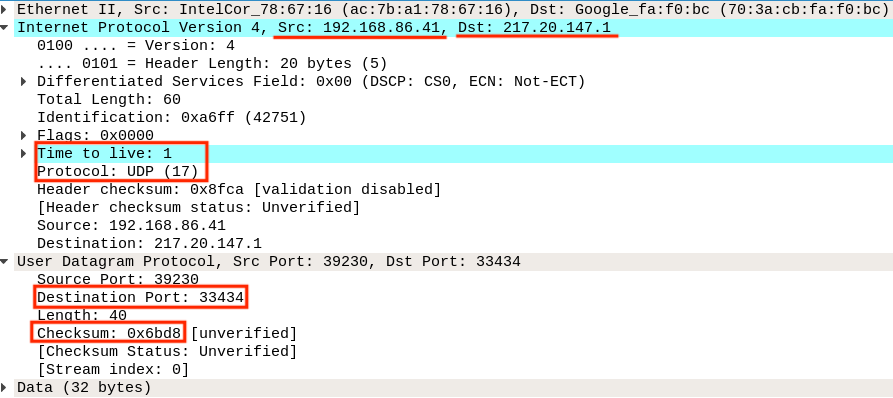
\includegraphics[width=0.9\textwidth]{traceroute-udp1}
	\caption{Отправка \code{traceroute} UDP дейтаграммы на порт 33434}
	\label{fig:trace-udp1}
\end{figure}

\begin{figure}[H]
	\centering
	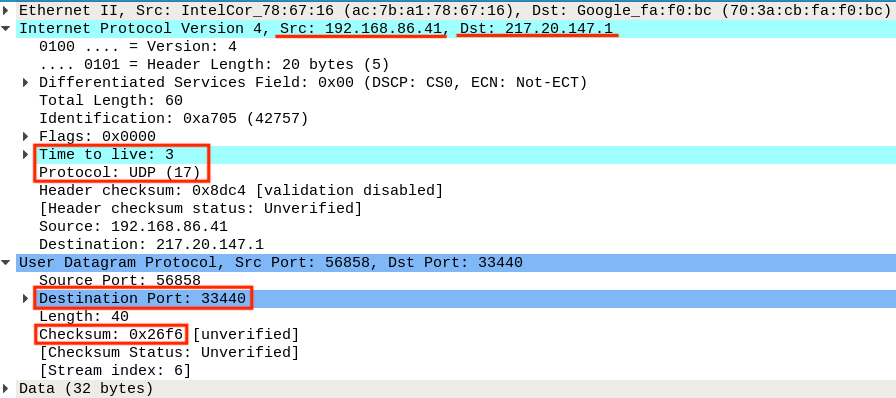
\includegraphics[width=0.9\textwidth]{traceroute-udp2}
	\caption{Отправка \code{traceroute} UDP дейтаграммы на порт 33440}
	\label{fig:trace-udp2}
\end{figure}

\begin{figure}[H]
	\centering
	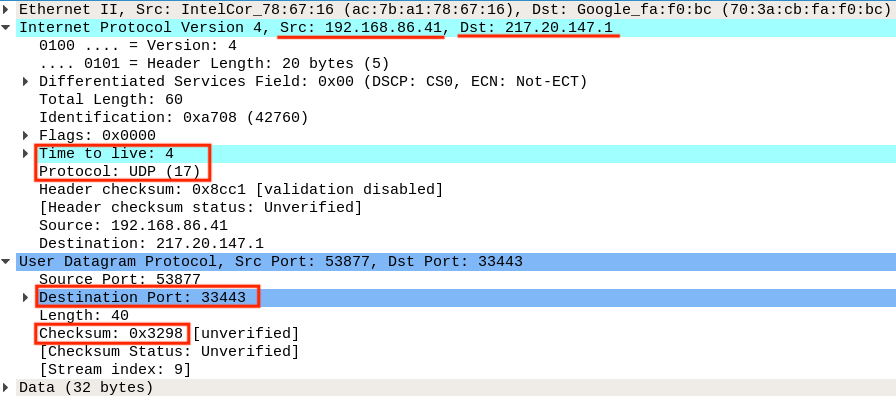
\includegraphics[width=0.9\textwidth]{traceroute-udp3}
	\caption{Отправка \code{traceroute} UDP дейтаграммы на порт 33443}
	\label{fig:trace-udp3}
\end{figure}

\begin{figure}[H]
	\centering
	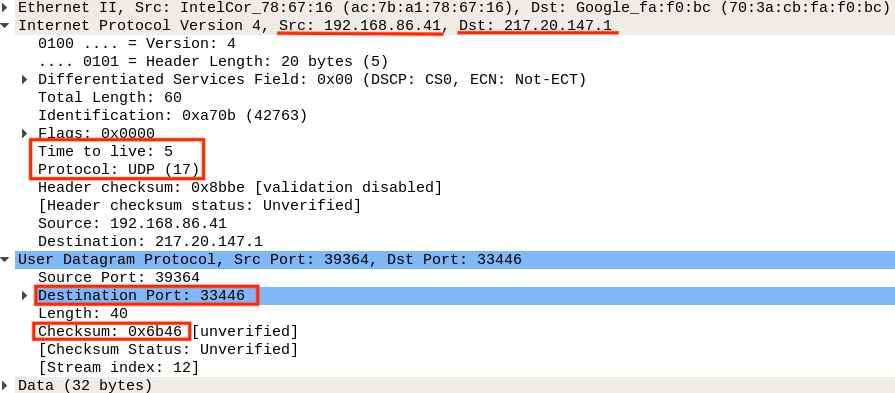
\includegraphics[width=0.9\textwidth]{traceroute-udp4}
	\caption{Отправка \code{traceroute} UDP дейтаграммы на порт 33446}
	\label{fig:trace-udp4}
\end{figure}

\subsection{Дополнение к опыту <<ping с фрагментацией>>}

На рис. \ref{fig:ping-list} представлен порядок отправки и получения IP пакетов.

\begin{figure}[H]
	\centering
	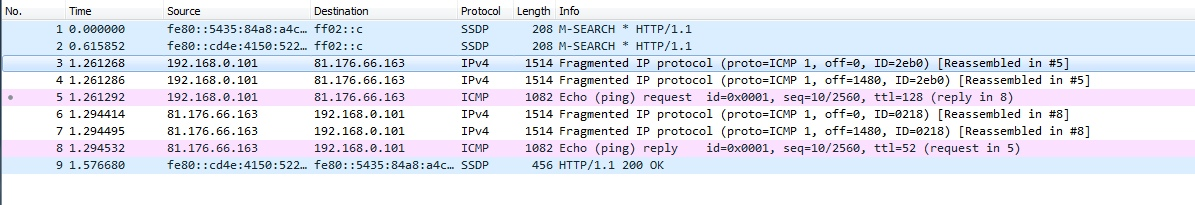
\includegraphics[width=0.9\textwidth]{ping-fraq-list}
	\caption{Порядок отправки и получения IP пакетов}
	\label{fig:ping-list}
\end{figure}

На рис. \ref{fig:ping-fraq-req-ip1} -- \ref{fig:ping-fraq-resp-ip2} изображены IP пакеты: первые 2 содержат фрагменты ICMP эхо-запроса, а вторые 2 содержат фрагменты ICMP эхо-ответа.

\begin{figure}[H]
	\centering
	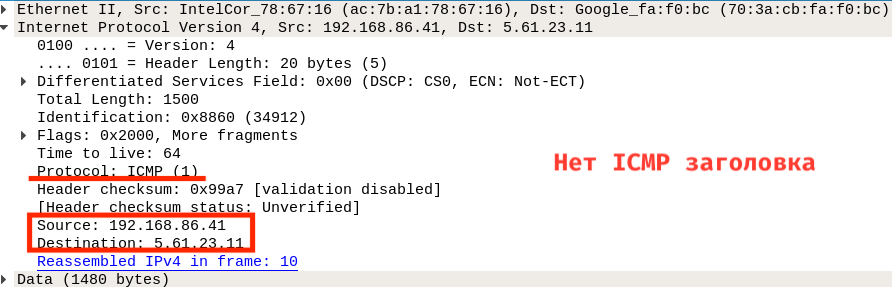
\includegraphics[width=0.9\textwidth]{ping-fraq-req-ip1}
	\caption{Перый фрагмент ICMP эхо-запроса}
	\label{fig:ping-fraq-req-ip1}
\end{figure}

\begin{figure}[H]
	\centering
	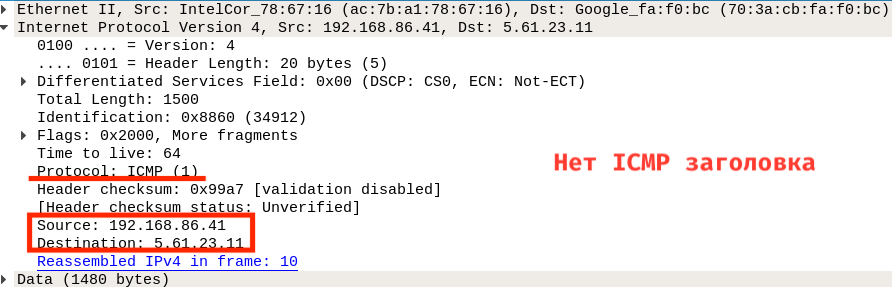
\includegraphics[width=0.9\textwidth]{ping-fraq-req-ip1}
	\caption{Второй фрагмент ICMP эхо-запросав}
	\label{fig:ping-fraq-req-ip2}
\end{figure}

\begin{figure}[H]
	\centering
	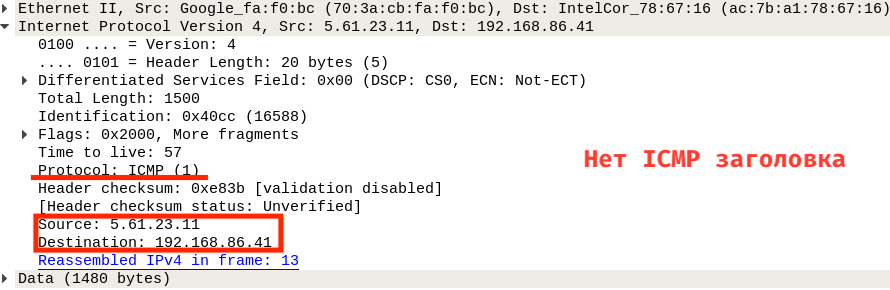
\includegraphics[width=0.9\textwidth]{ping-fraq-resp-ip1}
	\caption{Перый фрагмент ICMP эхо-ответа}
	\label{fig:ping-fraq-resp-ip1}
\end{figure}

\begin{figure}[H]
	\centering
	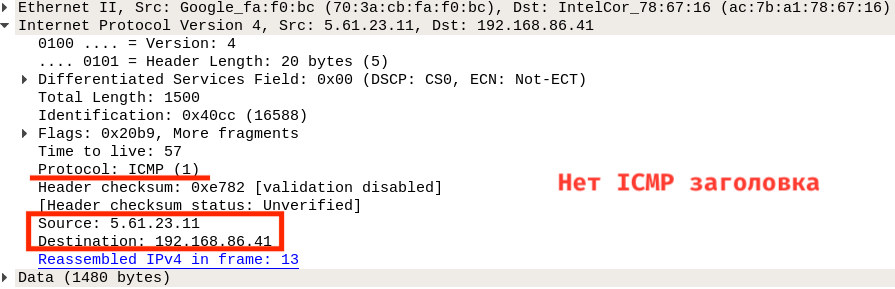
\includegraphics[width=0.9\textwidth]{ping-fraq-resp-ip2}
	\caption{Второй фрагмент ICMP эхо-ответа}
	\label{fig:ping-fraq-resp-ip2}
\end{figure}

Как в случае ICMP эхо-запроса, так и в случае ICMP эхо ответа, ICMP заголовок находится в третьем, т.е. последнем, IP фрагменте.

\end{document}
